The two major categories of cartography are general cartography and thematic cartography, which are introduced in chapter \ref{s:cartography} on page \pageref{s:cartography}. This categorization can be directly mapped from cartography to maps. The main objective of this chapter is to give an overview of different thematic maps and their usage. These maps can be subdivided into univariate and multivariate maps.

\subsubsubsection{Univariate Thematic Map Types}
Univariate maps are only dependent on one variable, except for the map variables like latitude and longitude and suchlike.

\sectionparagraph{Dot density map}
The first dot map in history is shown in figure \ref{fig:cholera-map} on page \pageref{fig:cholera-map}. It was the first map of its kind and could help in the display of disease outbreaks. This type of univariate thematic map uses points or dots to map discrete data. Attribute values of the given data determine the number of dots displayed in a specific regions. All dots need to be the same size. To explain the two different types of dot maps, imagine a dataset of customers where each customer has a location:

\begin{enumerate}
\ditem{One-to-one} \hfill \\
Each dot on the map represents exactly one item of the represented theme. Considering the example dataset mentioned above, every customer would be represented by exactly one dot.
\ditem{One-to-many} \hfill \\
Each dot on the map represents an aggregate of information. Therefore this type of dot map could be used with the aggregation of customers in a specific location. Thus the map maker needs to make the decision how many customers are aggregated, or rather how many customers are represented by one dot.
\end{enumerate}

Both types of dot density maps share the purpose, that they are not a tool to determine exact quantities. Getting the exact amount of dots in a high density area is a very cumbersome task and users often tend to underestimate dot totals as density increases \iacite{McMaster2001}. However, it is a very common technique for viewing the clustering, dispersion, linearity, and general pattern of a distribution. The technique appeared first in the 19\textsuperscript{th} century and is today accepted as one of the primary techniques for representing geographic patterns \iacite{Tyner2010}.

The map maker can use dots in a dot density map with a different type of level of detail. This means, that dots do not necessarily need to have an exact location. If he or she wants to discover a pattern on a state-wide level of detail, dots can be placed anywhere in their corresponding states, as long as they do not leave their state boundaries.
Another location based decision the map maker needs to make is, if the dots should use some kind of pseudo-random placement in case of overlapping. This decision is based on a maximum overlap constraint. It can be thought of as a random placement of dots in a square without violating the constraint.

According to \citeauthor{Tyner2010}, ther are some main design principles for dot maps that should be considered:
\begin{itemize}
\item The size of the dot.
\item The value assigned to the dot. This also includes the correct use of the two different types of dot maps.
\item The location of the dot on the map in case of an aggregated level of detail of the map.
\item The aggregated units in case of a one-to-many dot map. This design principle can be thought of as using a legend in order to tell the aggregated value one dot represents.
\end{itemize}
Changing any one of these can change the overall appearance and interpretation of the map \iacite{Tyner2010}.

The main advantage of this type of map is the understandability. It requires little to no cognitive effort by the user to read the map when compared to other types. Specific advantages of dot maps are the good measure of density and the loose coupling between the size of a dot and its represented value.
However, reading specific information from those maps is not an easy task as mentioned before. Additionally, if a map uses some kind of random placement without any hint in the visualization, map readers may potentially infer the locations of dots as precise locations of the mapped phenomenon. To counteract the second drawback, dot density maps with random placement of dots should consider the acual occurence of the mapped phenomenon, e.g. dots should not be placed in lakes for a map of population.

\sectionparagraph{Graduated symbol or proportional symbol map}
Figure \ref{fig:first-mixture} on page \pageref{fig:first-mixture} shows a special kind of a proportional symbol map. According to figure \ref{fig:va-channels} on page \pageref{fig:va-channels}, this type of map uses the visual channel of size to represent differences of discrete data. Again, this type of map can be subdivided into two categories: classed and unclassed. Classed ones are known as range-graded or graduated symbol maps, whereas unclassed ones are called proportional symbol maps. The latter one uses a symbol size proportional to the value of the attribute being mapped \iacite{Dutton.2014}.
Although circles are the most typical symbol used, it is possible to use any type of symbol, ranging from abstract, geometric symbols to pictographic symbols. Figure \ref{fig:different-symbols} on page \pageref{fig:different-symbols} shows two proportional symbol maps showing the same phenomenon. The left part of this figure uses the common circle as symbol, while the right side uses a pictogram. Albeit the established circle because of their compactness due to their low perimeter to area ratio, \citeauthor{Dutton.2014} says, that squares or bars are easier to estimate the size of the symbol.


\begin{figure}[!htb]
\centering
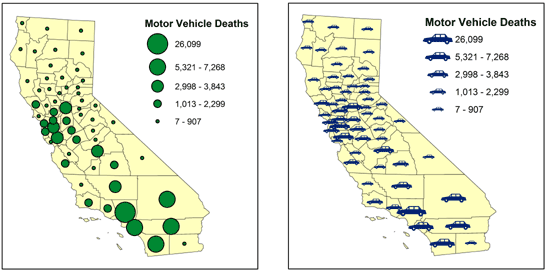
\includegraphics[height=5cm,keepaspectratio]{images/psm/symbols.png}
\caption[
    Two types of proportional symbol maps with different symbols \iacite{Dutton.2014}.
]{Two types of proportional symbol maps with different symbols.}
\label{fig:different-symbols}
\end{figure}

Another consideration in terms of symbol used is the fact, that squares and bars tend to run off the page with large values earlier than circles might \iacite{Dutton.2014}. \citeauthor{FLANNERY1971} introduced a scaling factor for proportional circles for better estimation of the value. However, this correction may not be very effective, because the correction itself does not consider the map context. A phenomenon related to the importance of context is known as the ebbinghaus illusion. Figure \ref{fig:ebbinghaus} on \pageref{fig:ebbinghaus} shows such an illusion. Both central circles actually have the same size, but because of the context of each side, the central circles appear different.

\begin{figure}[!htb]
\centering
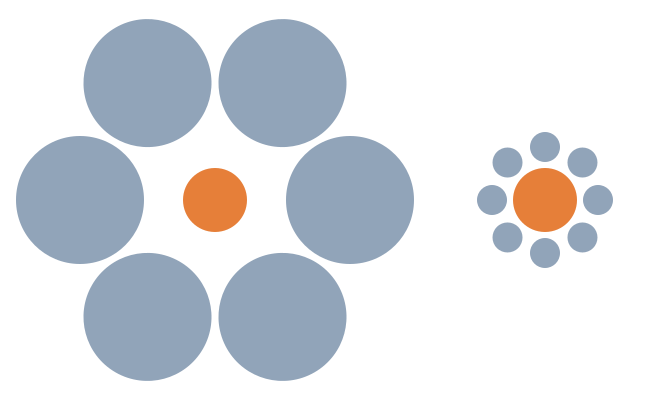
\includegraphics[height=5cm,keepaspectratio]{images/psm/ebbinghaus.png}
\caption[
    Ebbinghaus illusion, Urldate: 07.2016 \newline
    \small\texttt{\url{https://upload.wikimedia.org/wikipedia/commons/b/bc/Mond-vergleich.svg}}
]{Ebbinghaus illusion}
\label{fig:ebbinghaus}
\end{figure}

In order to combat the problem of value estimation, there are two major choices:
\begin{enumerate}
\item A legend could show proportional symbols which represent the different values of the mapped phenomenon. One possibility would be to display the smallest symbol, the largest symbol and some symbols at intermediate values.
\item Another alternative is to use range-graded symbols. Therefore the data needs to be classified, but in exchange the estimation problem is completly avoided. This alternative still needs consideration in the size of symbols, because each symbol should still be differentiable from each other.
\end{enumerate}

Based on the given knowledge about proportional and gradient symbol maps, it is possible to derive some main design principles:
\begin{itemize}
\item The estimation of the value of a symbol is key for this type of map. This is most easily accomplished with geometric symbols.
\item Use a legend with exmaples to increase the reader's ability to correctly estimate the value of a symbol.
\end{itemize}

A close related problem to the user's estimation problem is the actual scaling technique used. According to \citeauthor{Dent2008} the three most commong techniques used are
\begin{enumerate*}
\item absolute scaling,
\item apparent magnitude scaling and
\item range grading \iacite{Dent2008}.
\end{enumerate*}

\begin{enumerate}
\ditem{Absolute scaling} makes each symbol fit it's dat value on the scale being used. This means, that a symbol representing four items in a dataset is twice as big as a symbol representing two.
\ditem{Apparent magnitude scaling} compensates for human error interpretation in scale. Using this technique, a symbol having twice as much in value is not twice as big, because it would appear smaller, leading to interpretation error. This type of scaling takes this error into account and increased the size of a symbol by more than the proportional amount \iacite{Krygier.2007}.
\ditem{Range grading} classifies the data into a fixed amount of groups. Each group has a fixed range of values and the same symbol to represent. The groups only differ in the range of values they represent and the size of the symbols.
\end{enumerate}

The main advantage of a proportional symbol map is the flexibility it comes along with. Possible data can either be numerical or categorical nature. Even the way the data is used is adjustable. An item can be mapped on a precise location or to geographic areas, depending on the level of detail.
Comparing proportional symbol maps with dot density maps, one advantage is observable: the estimation problem of dot density maps is less tedious. However, if proportional symbol maps are put in comparison with choropleth maps, they also have an advantage: the size of the enumeration unit does not matter. This problem will be explained in detail in chapter \ref{s:choropleth} on page \pageref{s:choropleth}.

\sectionparagraph{Choropleth map}
Choropleth maps are extremely popular, probably the most common thematic map in use today. That's good because it means your audience is likely to understand them. One reason they're popular is that much of our geodata is reported by enumeration units, such as census data, and so we are accustomed to thinking of the world as divided into spatial units like census tracts, counties, and provinces. However, most cartographers would argue choropleth maps are over-used and commonly misused if the geographic phenomena being mapped aren't intrinsically tied to enumeration units: For example, communicable diseases, soil types, or age demographics don't care much about county lines or zip codes and rarely do they change abruptly at those human-created boundaries. By comparison, tax rates are very closely tied to enumeration units, do change abruptly, and make perfect sense as a choropleth map. The less the thing you are mapping is tied to enumeration units, the less sense a choropleth map makes.

These are maps, where areas are shaded according to a prearranged key, each shading or colour type representing a range of values. Population density information, expressed as 'per km²,' is appropriately represented using a choropleth map. Choropleth maps are also appropriate for indicating differences in land use, like the amount of recreational land or type of forest cover.



For continuous data, two mapping techniques are commonly used: choropleth and isarithmic mapping. This chapter will only cover choropleth mapping because the practical part of this thesis will not feature isarithmic mapping.


The choropleth method involves applying value or color
intensity to enumeration units (census tracts, counties, states, nations) based on some statistical
value. The higher an enumeration unit’s data value, the darker or more saturated the color value.
Fundamental to every choropleth method are the concepts of data standardization and
classification.
All choropleth data must be standardized. We repeat: a choropleth map may never – ever –
be used to map count data. If one maps raw data using the choropleth method, the visualization
will suffer from an inherent areal bias. Not all enumeration units are the same size; thus, some
enumeration units will naturally have more count data than others simply due to their areal
extent. For instance, Texas and California have greater populations than Rhode Island or
Connecticut. This should not be a surprise – Texas and California have huge areas compared to
the other two states. If you standardize the data by area, however, Connecticut and Rhode Island
are far more populated when it comes to the number of people per square kilometer. If you are
interested in comparing the raw number of people living in states, you should use proportional
symbols.
\label{s:choropleth}

\subsubsubsection{Multivariate Thematic Map Types}